\par \textbf{Теорема (Борсука–Улама–Люстерника–Шнирельмана):} $S^{n-1} \subset \mathbb{R}^n$ - сфера в $n$-мерном пространстве, $S^{n-1}=A_1 \cup \ldots \cup A_n$, $\forall i \: A_i$ - замкнуто или открыто. Тогда $\exists i, \: \exists \overline{x} \in A_i: \: -\overline{x} \in A_i$.

\par \textbf{Случай для $n=2$:} Пусть $S^1=A_1 \cup A_2$, $A_i$ - замкнутые (не обязательно связные). Тогда хотя бы одно из $A_i$ содержит диаметрально противоположные точки.
\par \Proof Рассмотрим произвольную точку $x \in A_1$. Если $-x \in A_1$, то все доказано. Иначе рассмотрим одну из дуг между этими точками и выберем $y \in A_1$ - последняя точка, которая лежит в $A_1$ (она существует, так как $A_1$ замкнуто). 
\begin{center}
    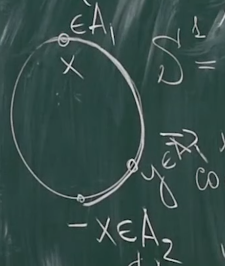
\includegraphics[scale=0.5]{images/dima_s1.png}
\end{center}

\par Пусть $y \not\in A_2$, тогда $y$ лежит в дополнении к $A_2$ вместе с какой-то окрестностью (в силу замкнутости $A_2$). Так как $y$ - последняя точка в $A_1$, то часть окрестности дальше $y$ не лежит ни в одном из $A_i$, что противоречит условию. Значит $y \in A_1 \cap A_2$. Так как $-y$ лежит на окружности, она обязана содержаться хотя бы в одном из $A_i$, значит, $y$ - искомая точка. \EndProof

\par \textbf{Случай для $n=3$, все $A_i$ замкнуты:} Предположим, что условие теоремы не выполнено. Тогда $diam \: A_i < 2$ (расстоение между самыми удаленными точками множества). Разобьем всю нашу сферу на кирпичики
\begin{center}
    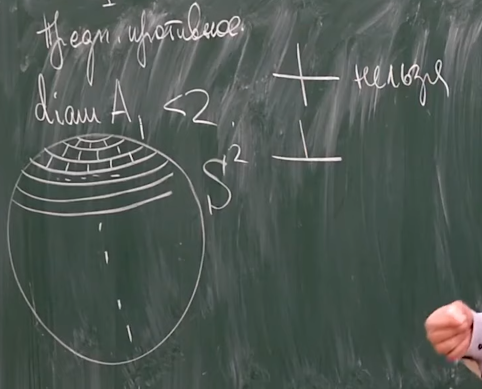
\includegraphics[scale=0.5]{images/dima_s2.png}
\end{center}

\par Рассмотрим объединение тех из них, которые пересекаются с $A_1$. Обозначим это объединение как $G_1$. Хотим подобрать размер кирпичиков так, чтобы $diam \: G_1 \leq diam \: A_1 + 2h < 2$, где $h$ - диаметр кирпичика. Тогда $\partial G_1=L_1\sqcup \ldots \sqcup L_k$, где $L_i$ - замкнутые несамопересекающиеся ломанные и $L_i \cap L_j=\varnothing$ (в силу того что $G_1$ состоит из кирпичиков). 

\par Рассмотрим $G_1'$ полученное из $G$ симметрией относительно центра сверы. $G_1 \cap G_1'=\varnothing$, так как $diam \: G_1 < 2$. $\partial G_1'=L_1' \sqcup \ldots \sqcup L_k'$. Ломанные $L_1, \ldots L_k, L_1', \ldots L_k'$ (они не пересекаются, так как полностью содержатся в $G_1$ или $G_1'$) разбивают сферу на $2k+1$ замкнутую связную часть (по теореме Жордана). В силу построения у каждой части есть симметричная ей относительно центра. Так как частей нечетное количество, то есть центрально симметричная часть. Так как в ней есть диаметрально противоположные точки, она не лежит полностью ни в $G_1$, ни в $G_1'$ и никак не пересекается с ними. Значит она не пересекается с $A_1 \subset G_1$. А отсюда следует, что она полностью покрывается $A_2 \cup A_3$. Теперь мы можем выделить в этой части замкнутую центрально симметричную кривую и свести задачу к двумерному случаю. $\square$